\section{\bfseries Korisnički interfejs}

U ovom poglavlju biće prikazano kako je zamišljen izgled korisničkog interfejsa naše aplikacije. Aplikaciju koriste zaposleni kao i korisnici. U narednim podsekcijama biće prikazane slike određenih delova aplikacije uz kratko objašnjenje. 

\subsection{\bfseries Registrovanje korisnika}

Način registrovanja korisnika je prikazan na sledećoj slici. Registrovanje se sastoji od unošenja korisničkog imena, imejla i lozinke.  Izvršava se klikom na dugme \say{Sign Up}.
\begin{figure}[H]
\begin{center}
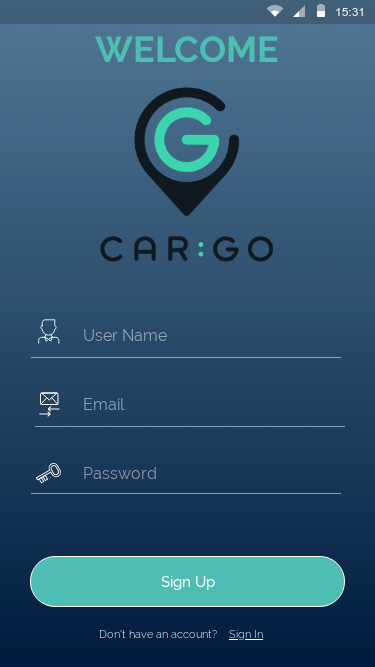
\includegraphics[width=7cm]{Slike/Registrovanje.png}
\end{center}
    \caption{Registrovanje korisnika.}
\label{fig:Registrovanje korisnika}
\end{figure}

\newpage
\subsection{\bfseries Prijavljivanje korisnika}

Prijavljivanje korisnika je dosta slično registrovanju, osim što u ovom slučaju nije potrebno unositi imejl, već samo korisničko ime i lozinko. Prijavljivanje se izvršava klikom na dugme \say{Sign In}.
\begin{figure}[H]
\begin{center}
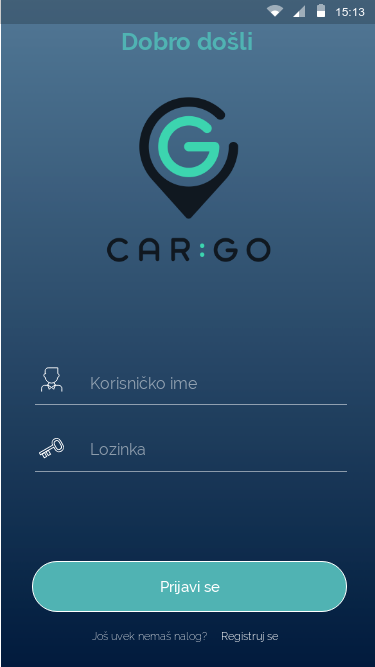
\includegraphics[width=7cm]{Slike/Prijavljivanje.png}
\end{center}
    \caption{Prijavljivanje korisnika.}
\label{fig:Prijavljivanje korisnika}
\end{figure}

\subsubsection{\bfseries Naručivanje vožnje}

U delu naručivanje vožnje, korisniku je putem interfejsa omogućeno da naruči vožnju. Korisnik to čini definisanjem lokacije na koju želi da bude odvežen. Nakon toga, aplikacija omogućava korisniku da vidi kolika bi iznosila cena vožnje kao i listu vozača koji su voljni da prihvate vožnju koju je korisnik zahtevao. Primer je prikazan kroz sliku ispod.

\begin{figure}[H]
\begin{center}
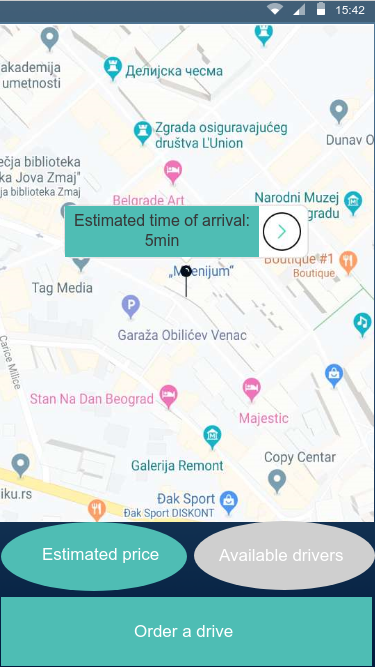
\includegraphics[width=7cm]{Slike/Narucivanje.png}
\end{center}
    \caption{Naručivanje vožnje.}
\label{fig:Naručivanje vožnje}
\end{figure}

\subsubsection{\bfseries Profil vozača}


\begin{figure}[H]
\begin{center}

\includegraphics[width=7cm]{Slike/Profil.png}
\end{center}
    \caption{Profil vozača.}
\label{fig:Profil vozača}
\end{figure}


